\documentclass{beamer}
%\usepackage{geometry}                % See geometry.pdf to learn the layout options. There are lots.
%\geometry{letterpaper}                   % ... or a4paper or a5paper or ... 
%\usepackage{setspace}
%\geometry{landscape}                % Activate for for rotated page geometry
%\usepackage[parfill]{parskip}    % Activate to begin paragraphs with an empty line rather than an indent
\usepackage{graphicx}

\usepackage{helvet}
\usepackage{nopageno}
\usetheme{keynote-black}

%\usepackage[german]{babel}
\usepackage[T1]{fontenc}
\usepackage[utf8]{inputenc}


\DeclareGraphicsRule{.tif}{png}{.png}{`convert #1 `dirname #1`/`basename #1 .tif`.png}

\title{Paintball}
\author{Leon Handreke}
\date{}                                           % Activate to display a given date or no date

\begin{document}
\frame{\titlepage}
\frame{\tableofcontents}

\section{What is Paintball?}

\frame{
  \frametitle{What is Paintball?}
  Wikipedia:
  \begin{quote}
    Paintball is a sport in which players compete to eliminate opponents by hitting them with pellets containing paint.
  \end{quote}
  \begin{itemize}
  \item Invented 1981, New Hampshire, UK 
  \end{itemize}
}

\section{Equipment}
\frame{
  \frametitle{Equipment}
  \begin{itemize}
    \item Marker
    \item Paintballs
    \item Clothing
  \end{itemize}
}

\frame{
  \frametitle{Marker}
  \begin{itemize}
  \item Speed of 90m/s, around 30km/h
  \item Powered by expanding gases
  \item Normally designed not to look like a real gun
  \end{itemize}
}

\frame{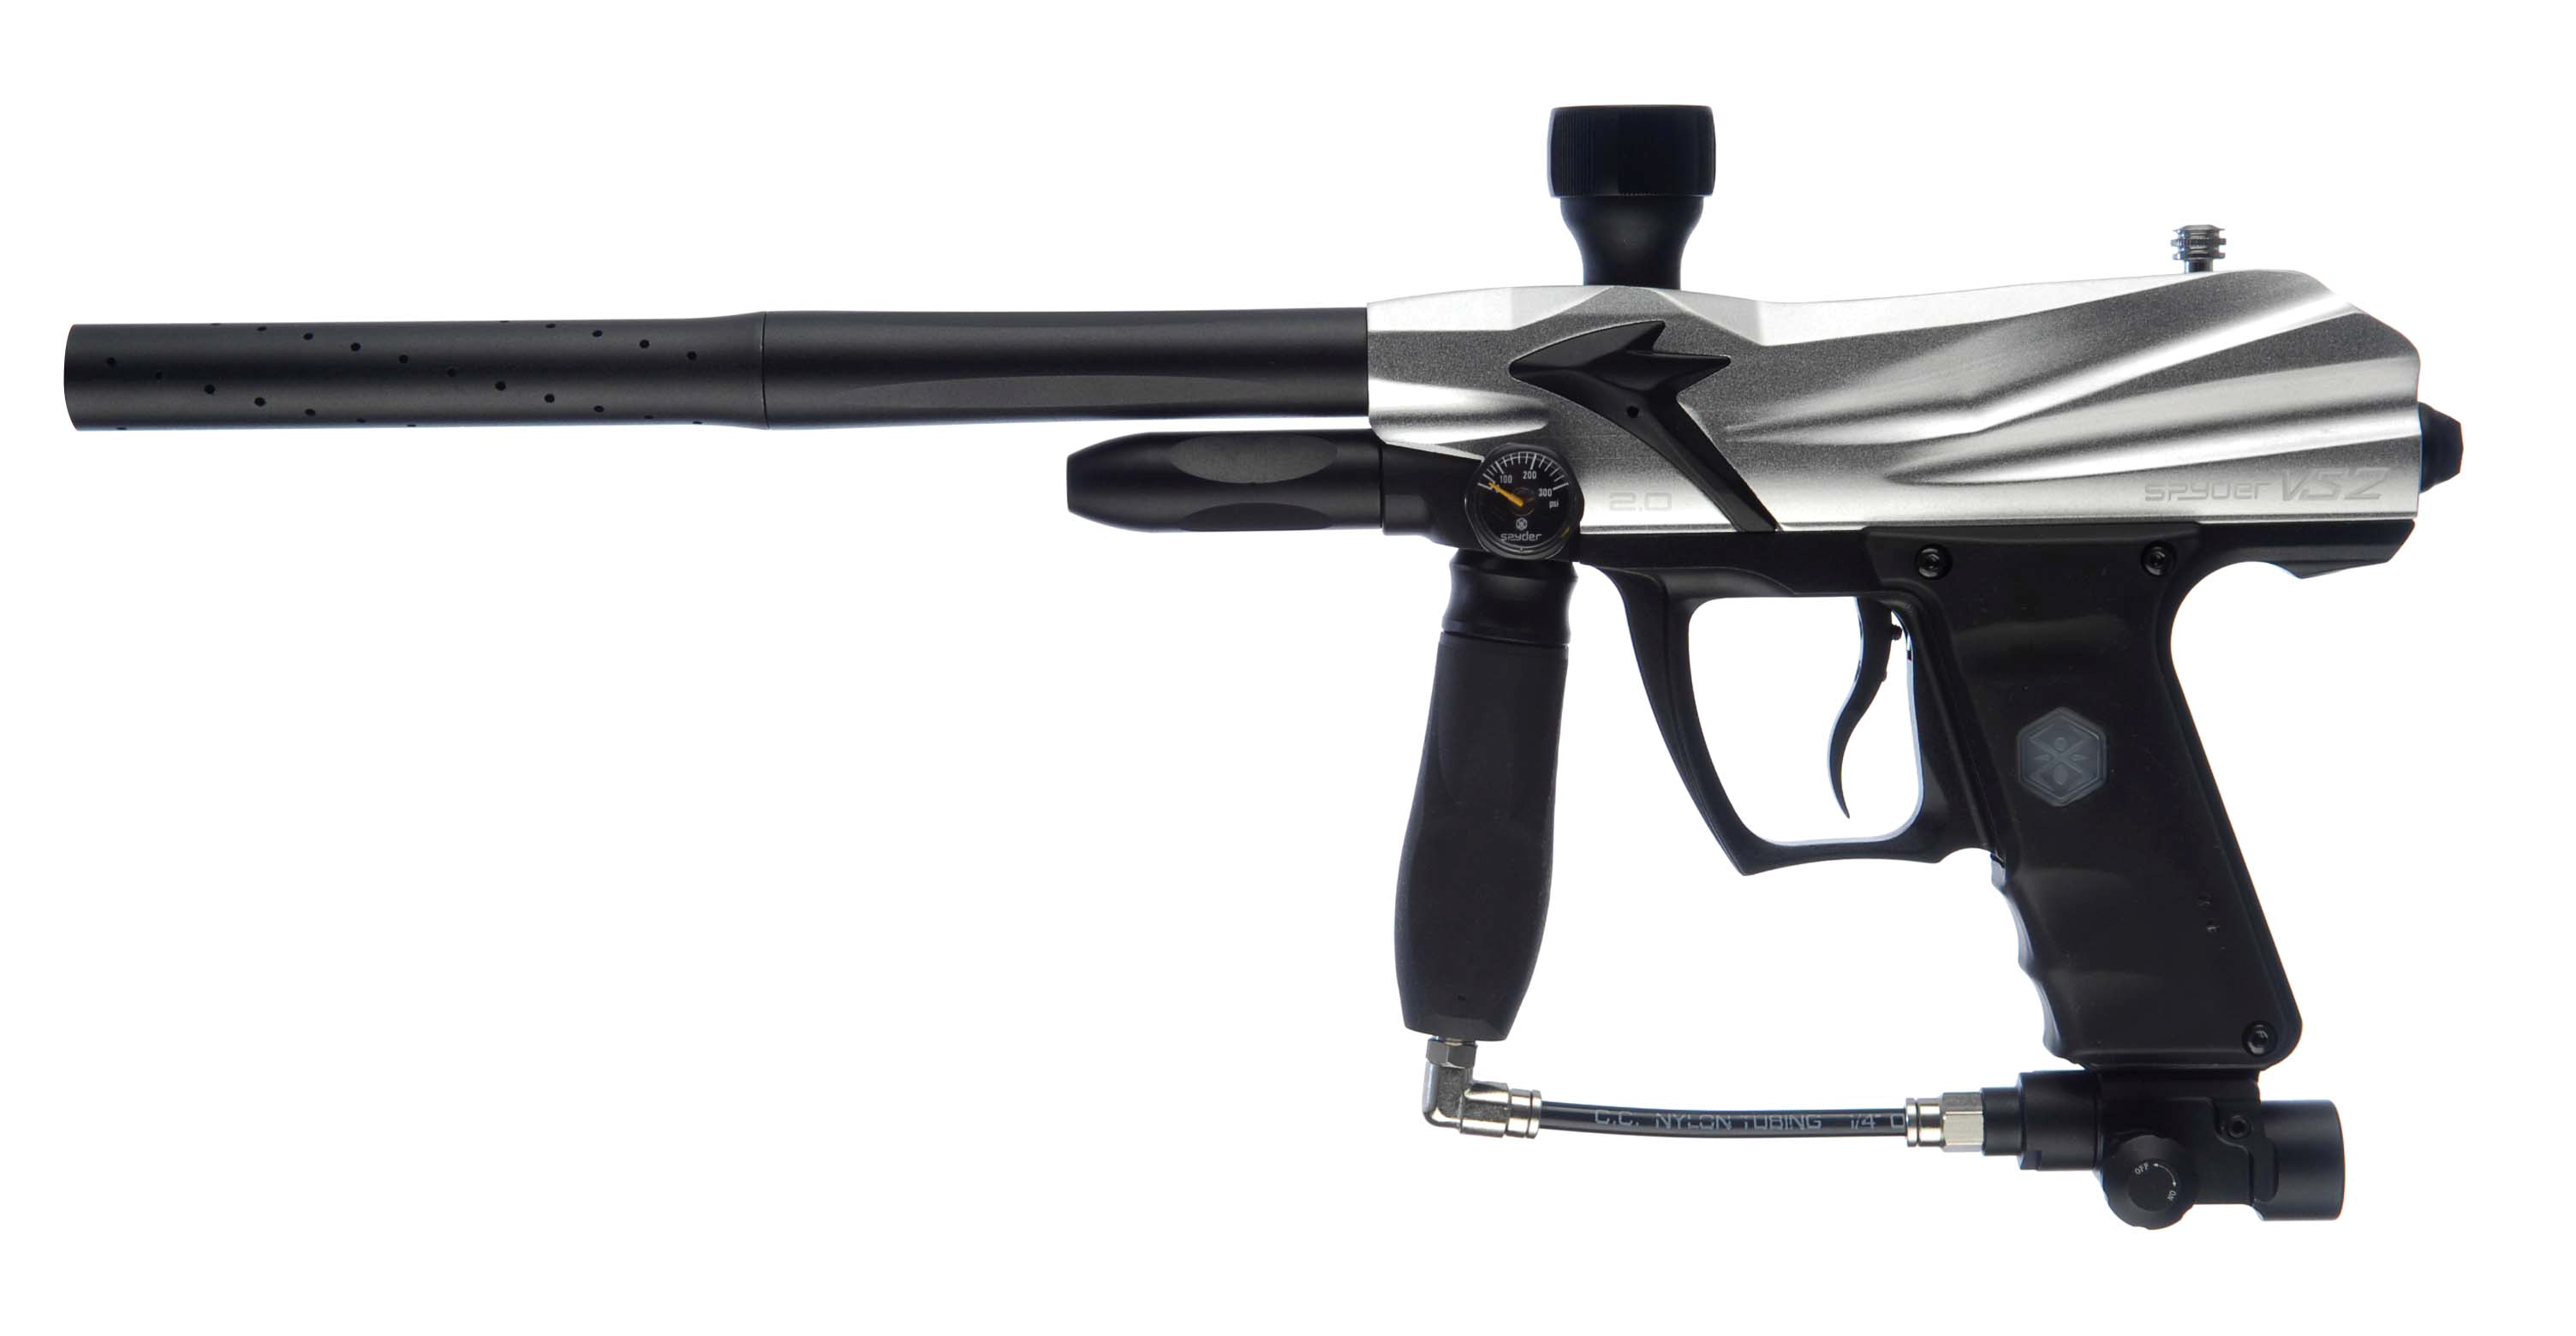
\includegraphics[width=1\textwidth]{marker}}
\frame{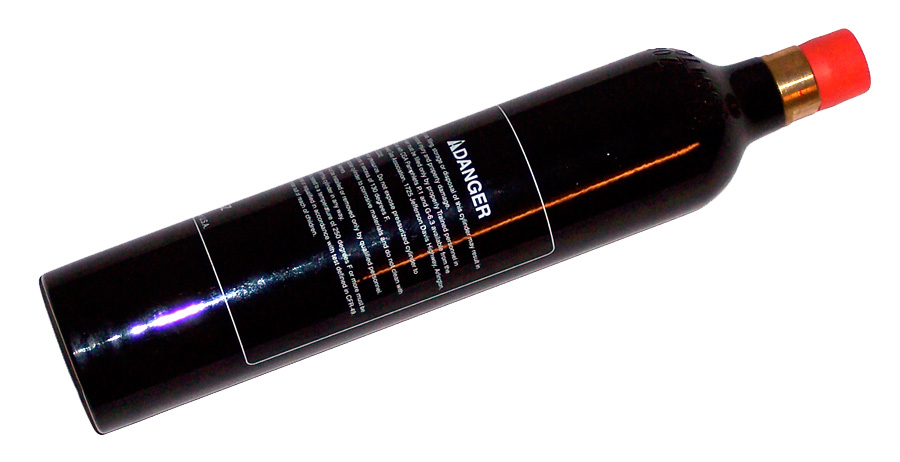
\includegraphics[width=1\textwidth]{air_tank}}
\frame{
  \frametitle{Paintballs}
  \begin{itemize}
  \item around .7 caliber (1.5cm)
  \item Cost: around 5 cents
  \item Different colors available (for different teams)
  \end{itemize}
}

\frame{
  \frametitle{Clothing}
  \begin{itemize}
  \item Mask
  \item (Camouflage) suit
  \item Baggy clothing to make paint ``bounce''
  \end{itemize}
}

\frame{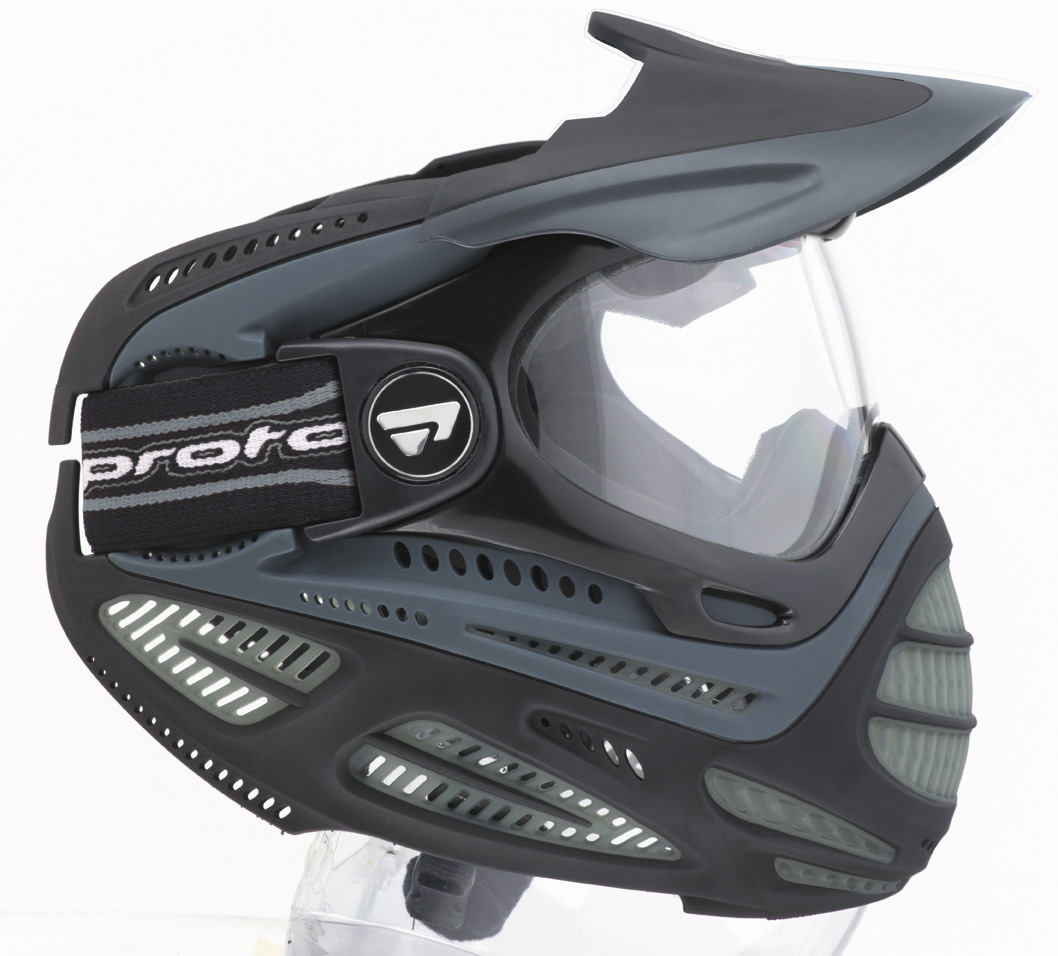
\includegraphics[height=0.9\textheight]{mask}}


\section{Rules}

\frame{
  \frametitle{Variations}
  \begin{itemize}
  \item Capture the Flag
  \item Slayer/Team Slayer
  \item Centerflag
  \end{itemize}
}

\frame{
  \frametitle{Rules}
  \begin{itemize}
  \item No Overshooting
  \item No Blind firing
  \item Max. Fire rate: 13.3 balls per second
  \end{itemize}
}

\section{Paintball Culture}

\frame{
  \frametitle{Paintball Culture}
  \begin{itemize}
  \item Non-militaristic
  \item Code of honour
  \item Sport aspect emphasized
  \item High safety
  \item Good organisation - Leagues, World Cup, Teams
  \end{itemize}
}

\section{Legality}

\frame{
  \frametitle{Legality}
  \begin{itemize}
  \item Banned in some American cities (e.g. Minneapolis)
  \item Plans for ban in Germany, May 2009 - Put on hold
  \end{itemize}
}

\frame{
  \frametitle{Why ban?}
  \begin{itemize}
  \item Trivialises violence/killing
  \item Militaristic aspect
  \end{itemize}
}

\frame{
  \frametitle{Pro Paintball!}
  \begin{itemize}
  \item Relieve stress
  \item Sport aspect
  \item Builds up anti-war attitude
  \item Economic aspect
  \item Ban youth culture?
  \item Where to draw the line?
  \end{itemize}
}

\frame{\maketitle}

\end{document}  
